% Options for packages loaded elsewhere
\PassOptionsToPackage{unicode}{hyperref}
\PassOptionsToPackage{hyphens}{url}
%
\documentclass[
]{book}
\usepackage{amsmath,amssymb}
\usepackage{lmodern}
\usepackage{iftex}
\ifPDFTeX
  \usepackage[T1]{fontenc}
  \usepackage[utf8]{inputenc}
  \usepackage{textcomp} % provide euro and other symbols
\else % if luatex or xetex
  \usepackage{unicode-math}
  \defaultfontfeatures{Scale=MatchLowercase}
  \defaultfontfeatures[\rmfamily]{Ligatures=TeX,Scale=1}
\fi
% Use upquote if available, for straight quotes in verbatim environments
\IfFileExists{upquote.sty}{\usepackage{upquote}}{}
\IfFileExists{microtype.sty}{% use microtype if available
  \usepackage[]{microtype}
  \UseMicrotypeSet[protrusion]{basicmath} % disable protrusion for tt fonts
}{}
\makeatletter
\@ifundefined{KOMAClassName}{% if non-KOMA class
  \IfFileExists{parskip.sty}{%
    \usepackage{parskip}
  }{% else
    \setlength{\parindent}{0pt}
    \setlength{\parskip}{6pt plus 2pt minus 1pt}}
}{% if KOMA class
  \KOMAoptions{parskip=half}}
\makeatother
\usepackage{xcolor}
\usepackage{color}
\usepackage{fancyvrb}
\newcommand{\VerbBar}{|}
\newcommand{\VERB}{\Verb[commandchars=\\\{\}]}
\DefineVerbatimEnvironment{Highlighting}{Verbatim}{commandchars=\\\{\}}
% Add ',fontsize=\small' for more characters per line
\usepackage{framed}
\definecolor{shadecolor}{RGB}{248,248,248}
\newenvironment{Shaded}{\begin{snugshade}}{\end{snugshade}}
\newcommand{\AlertTok}[1]{\textcolor[rgb]{0.94,0.16,0.16}{#1}}
\newcommand{\AnnotationTok}[1]{\textcolor[rgb]{0.56,0.35,0.01}{\textbf{\textit{#1}}}}
\newcommand{\AttributeTok}[1]{\textcolor[rgb]{0.77,0.63,0.00}{#1}}
\newcommand{\BaseNTok}[1]{\textcolor[rgb]{0.00,0.00,0.81}{#1}}
\newcommand{\BuiltInTok}[1]{#1}
\newcommand{\CharTok}[1]{\textcolor[rgb]{0.31,0.60,0.02}{#1}}
\newcommand{\CommentTok}[1]{\textcolor[rgb]{0.56,0.35,0.01}{\textit{#1}}}
\newcommand{\CommentVarTok}[1]{\textcolor[rgb]{0.56,0.35,0.01}{\textbf{\textit{#1}}}}
\newcommand{\ConstantTok}[1]{\textcolor[rgb]{0.00,0.00,0.00}{#1}}
\newcommand{\ControlFlowTok}[1]{\textcolor[rgb]{0.13,0.29,0.53}{\textbf{#1}}}
\newcommand{\DataTypeTok}[1]{\textcolor[rgb]{0.13,0.29,0.53}{#1}}
\newcommand{\DecValTok}[1]{\textcolor[rgb]{0.00,0.00,0.81}{#1}}
\newcommand{\DocumentationTok}[1]{\textcolor[rgb]{0.56,0.35,0.01}{\textbf{\textit{#1}}}}
\newcommand{\ErrorTok}[1]{\textcolor[rgb]{0.64,0.00,0.00}{\textbf{#1}}}
\newcommand{\ExtensionTok}[1]{#1}
\newcommand{\FloatTok}[1]{\textcolor[rgb]{0.00,0.00,0.81}{#1}}
\newcommand{\FunctionTok}[1]{\textcolor[rgb]{0.00,0.00,0.00}{#1}}
\newcommand{\ImportTok}[1]{#1}
\newcommand{\InformationTok}[1]{\textcolor[rgb]{0.56,0.35,0.01}{\textbf{\textit{#1}}}}
\newcommand{\KeywordTok}[1]{\textcolor[rgb]{0.13,0.29,0.53}{\textbf{#1}}}
\newcommand{\NormalTok}[1]{#1}
\newcommand{\OperatorTok}[1]{\textcolor[rgb]{0.81,0.36,0.00}{\textbf{#1}}}
\newcommand{\OtherTok}[1]{\textcolor[rgb]{0.56,0.35,0.01}{#1}}
\newcommand{\PreprocessorTok}[1]{\textcolor[rgb]{0.56,0.35,0.01}{\textit{#1}}}
\newcommand{\RegionMarkerTok}[1]{#1}
\newcommand{\SpecialCharTok}[1]{\textcolor[rgb]{0.00,0.00,0.00}{#1}}
\newcommand{\SpecialStringTok}[1]{\textcolor[rgb]{0.31,0.60,0.02}{#1}}
\newcommand{\StringTok}[1]{\textcolor[rgb]{0.31,0.60,0.02}{#1}}
\newcommand{\VariableTok}[1]{\textcolor[rgb]{0.00,0.00,0.00}{#1}}
\newcommand{\VerbatimStringTok}[1]{\textcolor[rgb]{0.31,0.60,0.02}{#1}}
\newcommand{\WarningTok}[1]{\textcolor[rgb]{0.56,0.35,0.01}{\textbf{\textit{#1}}}}
\usepackage{longtable,booktabs,array}
\usepackage{calc} % for calculating minipage widths
% Correct order of tables after \paragraph or \subparagraph
\usepackage{etoolbox}
\makeatletter
\patchcmd\longtable{\par}{\if@noskipsec\mbox{}\fi\par}{}{}
\makeatother
% Allow footnotes in longtable head/foot
\IfFileExists{footnotehyper.sty}{\usepackage{footnotehyper}}{\usepackage{footnote}}
\makesavenoteenv{longtable}
\usepackage{graphicx}
\makeatletter
\def\maxwidth{\ifdim\Gin@nat@width>\linewidth\linewidth\else\Gin@nat@width\fi}
\def\maxheight{\ifdim\Gin@nat@height>\textheight\textheight\else\Gin@nat@height\fi}
\makeatother
% Scale images if necessary, so that they will not overflow the page
% margins by default, and it is still possible to overwrite the defaults
% using explicit options in \includegraphics[width, height, ...]{}
\setkeys{Gin}{width=\maxwidth,height=\maxheight,keepaspectratio}
% Set default figure placement to htbp
\makeatletter
\def\fps@figure{htbp}
\makeatother
\setlength{\emergencystretch}{3em} % prevent overfull lines
\providecommand{\tightlist}{%
  \setlength{\itemsep}{0pt}\setlength{\parskip}{0pt}}
\setcounter{secnumdepth}{5}
\usepackage{booktabs}
\ifLuaTeX
  \usepackage{selnolig}  % disable illegal ligatures
\fi
\usepackage[]{natbib}
\bibliographystyle{plainnat}
\IfFileExists{bookmark.sty}{\usepackage{bookmark}}{\usepackage{hyperref}}
\IfFileExists{xurl.sty}{\usepackage{xurl}}{} % add URL line breaks if available
\urlstyle{same} % disable monospaced font for URLs
\hypersetup{
  pdftitle={MEPS tutorials},
  pdfauthor={Mark Bounthavong},
  hidelinks,
  pdfcreator={LaTeX via pandoc}}

\title{MEPS tutorials}
\author{Mark Bounthavong}
\date{2023-07-22}

\usepackage{amsthm}
\newtheorem{theorem}{Theorem}[chapter]
\newtheorem{lemma}{Lemma}[chapter]
\newtheorem{corollary}{Corollary}[chapter]
\newtheorem{proposition}{Proposition}[chapter]
\newtheorem{conjecture}{Conjecture}[chapter]
\theoremstyle{definition}
\newtheorem{definition}{Definition}[chapter]
\theoremstyle{definition}
\newtheorem{example}{Example}[chapter]
\theoremstyle{definition}
\newtheorem{exercise}{Exercise}[chapter]
\theoremstyle{definition}
\newtheorem{hypothesis}{Hypothesis}[chapter]
\theoremstyle{remark}
\newtheorem*{remark}{Remark}
\newtheorem*{solution}{Solution}
\begin{document}
\maketitle

{
\setcounter{tocdepth}{1}
\tableofcontents
}
\hypertarget{about}{%
\chapter*{About}\label{about}}
\addcontentsline{toc}{chapter}{About}

This is a collection of tutorials that use data from the Agency for Healthcare Research and Quality (AHRQ) Medical Expenditure Panel Survey (MEPS).

These tutorials use \href{https://cran.r-project.org/}{R} and \href{https://posit.co/products/open-source/rstudio/}{RStudio} for data loading, manipulation, analysis, and presentation.

Chapter 1 provides an introduction on how to load and import the data into R.

\hypertarget{introduction}{%
\chapter{Introduction}\label{introduction}}

The Agency for Healthcare Research and Quality (AHRQ) \href{https://www.meps.ahrq.gov/mepsweb/}{Medical Expenditure Panel Survey (MEPS)} is a set of data on U.S. households about their healthcare expenditures. It includes data on the individual / household demographics, socioeconomic status, insurance coverage, and healthcare expenditures. Healthcare expenditures include data on health-related spending, medical conditions, prescriptions, and utilization (e.g., number of office-based visits). MEPS draws upon a nationally representative subsample from the \href{https://www.cdc.gov/nchs/nhis/index.htm?CDC_AA_refVal=https\%3A\%2F\%2Fwww.cdc.gov\%2Fnchs\%2Fnhis.htm}{National Health Interview Survey}, which is conducted by the \href{https://www.cdc.gov/nchs/index.htm}{National Center for Health Statistics}. Hence, MEPS provides researchers with the ability to generate estimates for the representative U.S. population.

\hypertarget{meps-data}{%
\section{MEPS Data}\label{meps-data}}

MEPS data are located on their website in their \href{https://www.meps.ahrq.gov/mepsweb/data_stats/download_data_files.jsp}{data files page}. You can find data from 1996 to the most recent available year (during the writing of this tutorial, 2020 was the latest release).

\begin{figure}
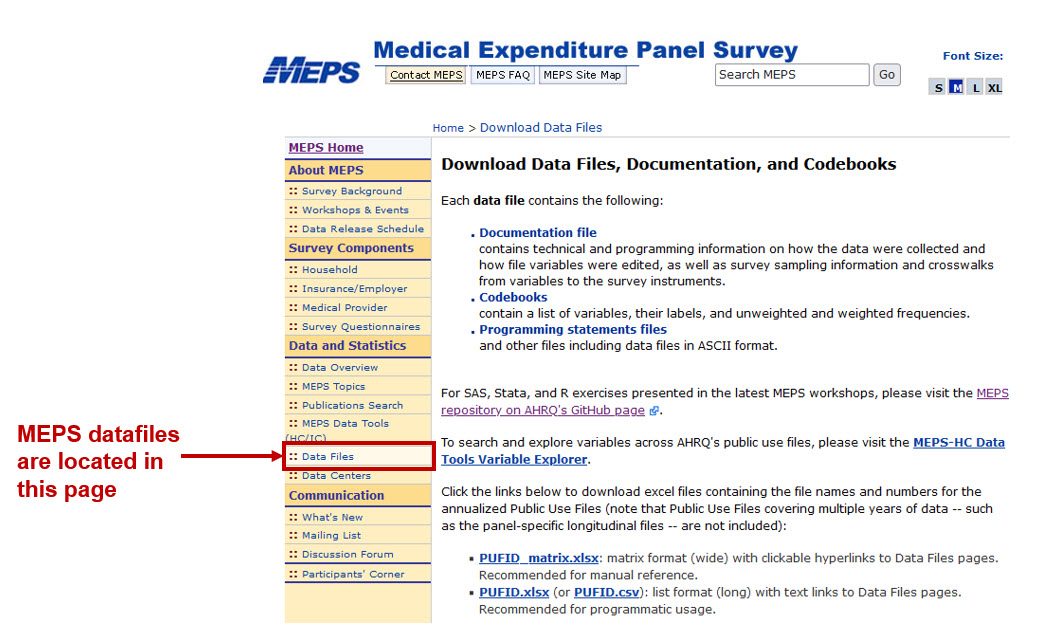
\includegraphics[width=1\linewidth]{Figure 1} \caption{Figure 1 - Location of MEPS data files}\label{fig:unnamed-chunk-2}
\end{figure}

The MEPS data files include the \href{https://www.meps.ahrq.gov/mepsweb/data_stats/download_data_files_detail.jsp?cboPufNumber=HC-224}{Full-Year Consolidated Data files}, which is the calendar-year summary of the different longitudinal panels. The Full-Year Consolidated Data files contain information on the annual healthcare expenditures by the type of care; it contains data on spending, insurance coverage, health status, patient satisfaction, and several health conditions. The Full-Year Consolidated Data files also contains information from several surveys (e.g,. Diabetes Care Survey).

\begin{figure}
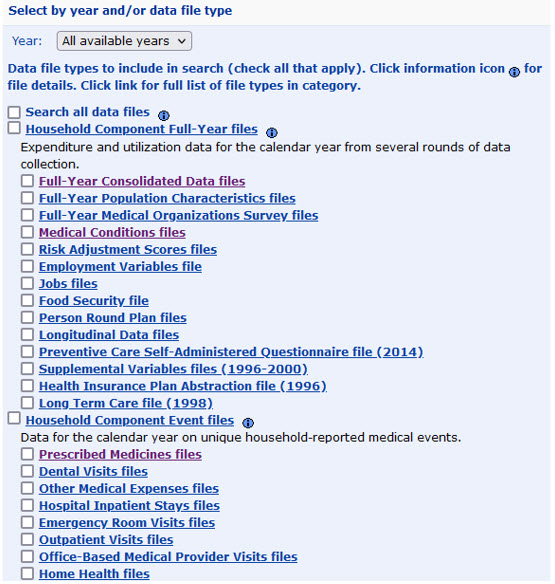
\includegraphics[width=1\linewidth]{Figure 2} \caption{Figure 2 - Full-Year Consolidated Data files and other data types}\label{fig:unnamed-chunk-3}
\end{figure}

\hypertarget{load-meps-data-into-r}{%
\section{Load MEPS data into R}\label{load-meps-data-into-r}}

MEPS data can be downloaded onto your local storage and read into a statistical software program such as Stata or R. But you can also communicate directly with the AHRQ MEPS website to load your data rather than having to download it. We will load the Full-Year Consolidated Data file from 2020, which is named \texttt{HC-224}. To find out the name of the file, you will need to go MEPS data files site and click on the Full-Year Consolidated Data files. In this page (Figure 2), you can see the data file with the code \texttt{HC-224}, which is the Full-Year Consolidated Data file for 2020. When we enter this into our R code, we will use the file name \texttt{h224}.

\begin{figure}
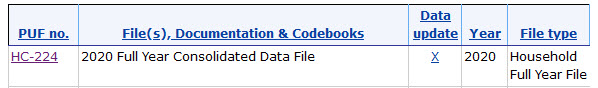
\includegraphics[width=1\linewidth]{Figure 3} \caption{Figure 3 - H224 is the MEP 2020 Full-Year Consolidated Data file.}\label{fig:unnamed-chunk-4}
\end{figure}

You will need to download and install the \href{https://github.com/e-mitchell/meps_r_pkg}{\texttt{MEPS} package}. The \texttt{MEPS} package will provide tools for you to load and manipulate the MEPS Data files. You will need to have R \texttt{devtools} package installed.

\begin{Shaded}
\begin{Highlighting}[]
\DocumentationTok{\#\# Install the devtools package}
\CommentTok{\# install.packages("devtools") \#\# You only need to install this once}
\CommentTok{\# library("devtools")  \#\# You will need to reload the MEPS package each time you restart R}
\CommentTok{\# install\_github("e{-}mitchell/meps\_r\_pkg/MEPS") \#\# This will install the MEPS package for R}
\end{Highlighting}
\end{Shaded}

There are two methods to load MEPS data into R.

Method 1 requires that you know the file name. In this example, the MEPS 2020 Full-Year Consolidated Data file is named \texttt{h224}. We will use the \texttt{read\_MEPS} function to load the MEPS data onto R.

When using Method 2 to load the MEPS data, we don't need to know the file name, but we need to know the year and the data type. For example, for the Full-Year Consolidated Data file, we use the \texttt{year\ =\ 2020} and \texttt{type\ =\ "FYC"} option. For this method, we will also use the \texttt{read\_MEPS} function to the MEPS data onto R.

The \texttt{tolower} function is used to change all the variable names from upper case to lower case. MEPS defaults the column names to upper case. I like to change this to lower case because it's easier for me to type.

\begin{Shaded}
\begin{Highlighting}[]
\DocumentationTok{\#\#\# Load the MEPS package}
\FunctionTok{library}\NormalTok{(}\StringTok{"MEPS"}\NormalTok{) }\DocumentationTok{\#\# You need to load the library every time you restart R}

\DocumentationTok{\#\#\#\# Method 1: Load data from AHRQ MEPS website}
\NormalTok{hc2020 }\OtherTok{=} \FunctionTok{read\_MEPS}\NormalTok{(}\AttributeTok{file =} \StringTok{"h224"}\NormalTok{)}

\DocumentationTok{\#\#\#\# Method 2: Load data from AHRQ MEPS website}
\NormalTok{hc2020 }\OtherTok{=} \FunctionTok{read\_MEPS}\NormalTok{(}\AttributeTok{year =} \DecValTok{2020}\NormalTok{, }\AttributeTok{type =} \StringTok{"FYC"}\NormalTok{)}

\DocumentationTok{\#\# Change column names to lowercase}
\FunctionTok{names}\NormalTok{(hc2020) }\OtherTok{\textless{}{-}} \FunctionTok{tolower}\NormalTok{(}\FunctionTok{names}\NormalTok{(hc2020))}
\end{Highlighting}
\end{Shaded}

There are over 1400 variables in the MEPS 2020 Full-Year Consolidated Data file. We can reduce this to the essential variables using the \texttt{subset} function. This will generate a smaller data frame that we will call \texttt{keep\_meps}. The variables that we want to collect are the subject unique identifier (\texttt{dupersid}), the survey weights (\texttt{varpsu}, \texttt{varstr}, \texttt{perwt20f}), and the total healthcare expenditures for 2020 (\texttt{totexp20}).

\begin{Shaded}
\begin{Highlighting}[]
\DocumentationTok{\#\#\# Keep the subject\textquotesingle{}s unique ID, survey weights, and total expenditures}
\NormalTok{keep\_meps }\OtherTok{\textless{}{-}} \FunctionTok{subset}\NormalTok{(hc2020, }\AttributeTok{select =} \FunctionTok{c}\NormalTok{(dupersid, varpsu, varstr, perwt20f, totexp20))}

\FunctionTok{head}\NormalTok{(keep\_meps) }\DocumentationTok{\#\# View the first six rows of the data frame}
\end{Highlighting}
\end{Shaded}

\begin{verbatim}
## # A tibble: 6 x 5
##   dupersid   varpsu varstr perwt20f totexp20
##   <chr>       <dbl>  <dbl>    <dbl>    <dbl>
## 1 2320005101      1   2079    8418.      459
## 2 2320005102      1   2079    5200.      564
## 3 2320006101      1   2028    2140.      140
## 4 2320006102      1   2028    2216.     4673
## 5 2320006103      1   2028    4157.      410
## 6 2320012102      2   2069    1961.     2726
\end{verbatim}

Since MEPS uses a complex survey design, these weights are needed to estimate standard errors that are reflective of the representative sample of the U.S. population. We'll learn how to apply these survey weights to the MEPS data files in a future tutorial.

\hypertarget{conclusions}{%
\section{Conclusions}\label{conclusions}}

Loading MEPS data into R allows us to perform analysis easily and quickly. In this tutorial, you learned how to load MEPS data into R directly from the MEPS website. However, you can also download the MEPS data onto your local storage and use the \texttt{setwd} command to set the working directory.

In future tutorials, we'll learn how to apply the survey weights and perform descriptive analyses using the MEPS data files.

\hypertarget{acknowledgements}{%
\section{Acknowledgements}\label{acknowledgements}}

There are a lot of tutorials on how to use MEPS data with R. I found the \href{https://github.com/HHS-AHRQ/MEPS}{AHRQ MEPS GitHub page} to be an invaluable resource.

This is a work in progress, and I may update this in the future.

\hypertarget{cross}{%
\chapter{Cross-references}\label{cross}}

Cross-references make it easier for your readers to find and link to elements in your book.

\hypertarget{chapters-and-sub-chapters}{%
\section{Chapters and sub-chapters}\label{chapters-and-sub-chapters}}

There are two steps to cross-reference any heading:

\begin{enumerate}
\def\labelenumi{\arabic{enumi}.}
\tightlist
\item
  Label the heading: \texttt{\#\ Hello\ world\ \{\#nice-label\}}.

  \begin{itemize}
  \tightlist
  \item
    Leave the label off if you like the automated heading generated based on your heading title: for example, \texttt{\#\ Hello\ world} = \texttt{\#\ Hello\ world\ \{\#hello-world\}}.
  \item
    To label an un-numbered heading, use: \texttt{\#\ Hello\ world\ \{-\#nice-label\}} or \texttt{\{\#\ Hello\ world\ .unnumbered\}}.
  \end{itemize}
\item
  Next, reference the labeled heading anywhere in the text using \texttt{\textbackslash{}@ref(nice-label)}; for example, please see Chapter \ref{cross}.

  \begin{itemize}
  \tightlist
  \item
    If you prefer text as the link instead of a numbered reference use: \protect\hyperlink{cross}{any text you want can go here}.
  \end{itemize}
\end{enumerate}

\hypertarget{captioned-figures-and-tables}{%
\section{Captioned figures and tables}\label{captioned-figures-and-tables}}

Figures and tables \emph{with captions} can also be cross-referenced from elsewhere in your book using \texttt{\textbackslash{}@ref(fig:chunk-label)} and \texttt{\textbackslash{}@ref(tab:chunk-label)}, respectively.

See Figure \ref{fig:nice-fig}.

\begin{Shaded}
\begin{Highlighting}[]
\FunctionTok{par}\NormalTok{(}\AttributeTok{mar =} \FunctionTok{c}\NormalTok{(}\DecValTok{4}\NormalTok{, }\DecValTok{4}\NormalTok{, .}\DecValTok{1}\NormalTok{, .}\DecValTok{1}\NormalTok{))}
\FunctionTok{plot}\NormalTok{(pressure, }\AttributeTok{type =} \StringTok{\textquotesingle{}b\textquotesingle{}}\NormalTok{, }\AttributeTok{pch =} \DecValTok{19}\NormalTok{)}
\end{Highlighting}
\end{Shaded}

\begin{figure}

{\centering 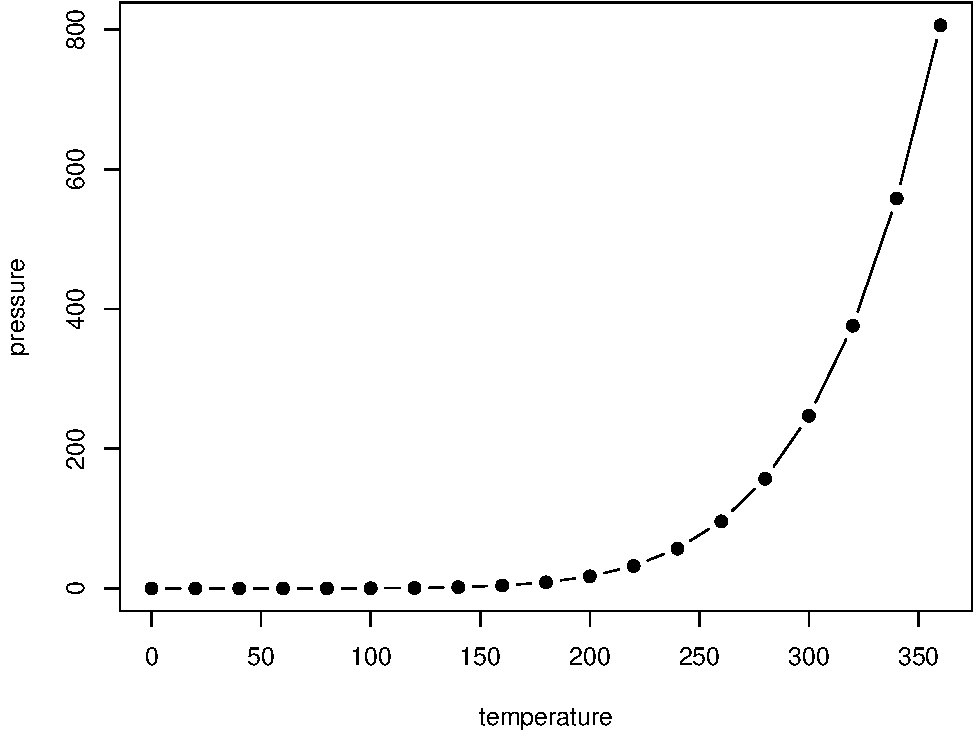
\includegraphics[width=0.8\linewidth]{_main_files/figure-latex/nice-fig-1} 

}

\caption{Here is a nice figure!}\label{fig:nice-fig}
\end{figure}

Don't miss Table \ref{tab:nice-tab}.

\begin{Shaded}
\begin{Highlighting}[]
\NormalTok{knitr}\SpecialCharTok{::}\FunctionTok{kable}\NormalTok{(}
  \FunctionTok{head}\NormalTok{(pressure, }\DecValTok{10}\NormalTok{), }\AttributeTok{caption =} \StringTok{\textquotesingle{}Here is a nice table!\textquotesingle{}}\NormalTok{,}
  \AttributeTok{booktabs =} \ConstantTok{TRUE}
\NormalTok{)}
\end{Highlighting}
\end{Shaded}

\begin{table}

\caption{\label{tab:nice-tab}Here is a nice table!}
\centering
\begin{tabular}[t]{rr}
\toprule
temperature & pressure\\
\midrule
0 & 0.0002\\
20 & 0.0012\\
40 & 0.0060\\
60 & 0.0300\\
80 & 0.0900\\
\addlinespace
100 & 0.2700\\
120 & 0.7500\\
140 & 1.8500\\
160 & 4.2000\\
180 & 8.8000\\
\bottomrule
\end{tabular}
\end{table}

\hypertarget{parts}{%
\chapter{Parts}\label{parts}}

You can add parts to organize one or more book chapters together. Parts can be inserted at the top of an .Rmd file, before the first-level chapter heading in that same file.

Add a numbered part: \texttt{\#\ (PART)\ Act\ one\ \{-\}} (followed by \texttt{\#\ A\ chapter})

Add an unnumbered part: \texttt{\#\ (PART\textbackslash{}*)\ Act\ one\ \{-\}} (followed by \texttt{\#\ A\ chapter})

Add an appendix as a special kind of un-numbered part: \texttt{\#\ (APPENDIX)\ Other\ stuff\ \{-\}} (followed by \texttt{\#\ A\ chapter}). Chapters in an appendix are prepended with letters instead of numbers.

\hypertarget{footnotes-and-citations}{%
\chapter{Footnotes and citations}\label{footnotes-and-citations}}

\hypertarget{footnotes}{%
\section{Footnotes}\label{footnotes}}

Footnotes are put inside the square brackets after a caret \texttt{\^{}{[}{]}}. Like this one \footnote{This is a footnote.}.

\hypertarget{citations}{%
\section{Citations}\label{citations}}

Reference items in your bibliography file(s) using \texttt{@key}.

For example, we are using the \textbf{bookdown} package \citep{R-bookdown} (check out the last code chunk in index.Rmd to see how this citation key was added) in this sample book, which was built on top of R Markdown and \textbf{knitr} \citep{xie2015} (this citation was added manually in an external file book.bib).
Note that the \texttt{.bib} files need to be listed in the index.Rmd with the YAML \texttt{bibliography} key.

The RStudio Visual Markdown Editor can also make it easier to insert citations: \url{https://rstudio.github.io/visual-markdown-editing/\#/citations}

\hypertarget{blocks}{%
\chapter{Blocks}\label{blocks}}

\hypertarget{equations}{%
\section{Equations}\label{equations}}

Here is an equation.

\begin{equation} 
  f\left(k\right) = \binom{n}{k} p^k\left(1-p\right)^{n-k}
  \label{eq:binom}
\end{equation}

You may refer to using \texttt{\textbackslash{}@ref(eq:binom)}, like see Equation \eqref{eq:binom}.

\hypertarget{theorems-and-proofs}{%
\section{Theorems and proofs}\label{theorems-and-proofs}}

Labeled theorems can be referenced in text using \texttt{\textbackslash{}@ref(thm:tri)}, for example, check out this smart theorem \ref{thm:tri}.

\begin{theorem}
\protect\hypertarget{thm:tri}{}\label{thm:tri}For a right triangle, if \(c\) denotes the \emph{length} of the hypotenuse
and \(a\) and \(b\) denote the lengths of the \textbf{other} two sides, we have
\[a^2 + b^2 = c^2\]
\end{theorem}

Read more here \url{https://bookdown.org/yihui/bookdown/markdown-extensions-by-bookdown.html}.

\hypertarget{callout-blocks}{%
\section{Callout blocks}\label{callout-blocks}}

The R Markdown Cookbook provides more help on how to use custom blocks to design your own callouts: \url{https://bookdown.org/yihui/rmarkdown-cookbook/custom-blocks.html}

\hypertarget{sharing-your-book}{%
\chapter{Sharing your book}\label{sharing-your-book}}

\hypertarget{publishing}{%
\section{Publishing}\label{publishing}}

HTML books can be published online, see: \url{https://bookdown.org/yihui/bookdown/publishing.html}

\hypertarget{pages}{%
\section{404 pages}\label{pages}}

By default, users will be directed to a 404 page if they try to access a webpage that cannot be found. If you'd like to customize your 404 page instead of using the default, you may add either a \texttt{\_404.Rmd} or \texttt{\_404.md} file to your project root and use code and/or Markdown syntax.

\hypertarget{metadata-for-sharing}{%
\section{Metadata for sharing}\label{metadata-for-sharing}}

Bookdown HTML books will provide HTML metadata for social sharing on platforms like Twitter, Facebook, and LinkedIn, using information you provide in the \texttt{index.Rmd} YAML. To setup, set the \texttt{url} for your book and the path to your \texttt{cover-image} file. Your book's \texttt{title} and \texttt{description} are also used.

This \texttt{gitbook} uses the same social sharing data across all chapters in your book- all links shared will look the same.

Specify your book's source repository on GitHub using the \texttt{edit} key under the configuration options in the \texttt{\_output.yml} file, which allows users to suggest an edit by linking to a chapter's source file.

Read more about the features of this output format here:

\url{https://pkgs.rstudio.com/bookdown/reference/gitbook.html}

Or use:

\begin{Shaded}
\begin{Highlighting}[]
\NormalTok{?bookdown}\SpecialCharTok{::}\NormalTok{gitbook}
\end{Highlighting}
\end{Shaded}


  \bibliography{book.bib,packages.bib}

\end{document}
